\documentclass[11pt, a4paper]{article}

\usepackage{amsmath}
\usepackage{amssymb}
\usepackage{amsfonts}
\usepackage{mathtools}

\usepackage[thmmarks, amsmath]{ntheorem}

\usepackage{graphicx}
\usepackage{float}

\usepackage{tikz-cd}
\usetikzlibrary{arrows, positioning, intersections}

\usepackage{diffcoeff}
\diffdef{}{op-symbol=\mathrm{d},op-order-sep=0mu}

\usepackage{cancel}
\usepackage{interval}
\usepackage{mleftright}

\usepackage[inline]{enumitem}
\SetEnumitemKey{algorithm}{label={Step \Roman*.}, ref=\Roman*, labelindent=0pt, labelsep=!, leftmargin=*, align=left,itemindent=0pt}
\setlist[enumerate,1]{label=\roman*)}

%\usepackage{cite}

\usepackage[utf8]{inputenc}
\usepackage[margin=3cm]{geometry}

%\setlist[enumerate,1]{label=\alph*)}

\title{Handout: Thesis Presentation\\
Computing Masliv Indices in Two Dimensions and\\
Filtered Floer Homology of a few Hamiltonians on the Torus}
\author{Author: Duarte Maia\\
Supervisor: Prof. Miguel Abreu}
\date{July 5, 2022}

\theorembodyfont{\upshape}
\theoremseparator{.}
\newtheorem{theorem}{Theorem}
\newtheorem{prop}{Proposition}
\renewtheorem*{prop*}{Proposition}
\newtheorem{lemma}{Lemma}
\newtheorem{conjecture}{Conjecture}
\newtheorem{idea}{Idea}
\theoremsymbol{\ensuremath{\square}}
\newtheorem{definition}{Definition}
\newtheorem{ex}{Example}

\theoremstyle{nonumberplain}
\theoremheaderfont{\itshape}
\theorembodyfont{\upshape}
\theoremseparator{:}
\theoremsymbol{\ensuremath{\blacksquare}}
\newtheorem{proof}{Proof}

\newcommand{\R}{\mathbb{R}}
\newcommand{\C}{\mathbb{C}}
\newcommand{\Z}{\mathbb{Z}}
\newcommand{\FF}{\mathbb{F}}

\newcommand{\PP}{\mathbb{P}}
\newcommand{\LL}{\mathrm{L}}
\renewcommand{\AA}{\mathrm{A}}
\newcommand{\BB}{\mathrm{B}}


\newcommand{\CF}{\mathrm{CF}}
\newcommand{\HF}{\mathrm{HF}}

\newcommand{\I}{\mathrm{i}}
\newcommand{\e}{\mathrm{e}}

\newcommand{\Ix}{\mathop{\mathrm{I\mkern0.7mu x}}}
%\newcommand{\Ix}{\mathop{\mathrm{ix}}}


\newcommand{\id}{\mathrm{id}}
\newcommand{\HH}{\mathrm{H}}


\DeclareMathOperator{\inte}{int}
\DeclareMathOperator{\codim}{codim}
\newcommand{\grad}{\nabla}
\newcommand{\into}{\mathbin{\lrcorner}}

\DeclarePairedDelimiter{\norm}{\lvert}{\rvert}
\DeclarePairedDelimiter{\Norm}{\lVert}{\rVert}
\DeclarePairedDelimiter{\abs}{\lvert}{\rvert}
\DeclarePairedDelimiter{\braket}{\langle}{\rangle}

\newcommand{\conj}[1]{\overline{#1}}
\newcommand{\transposed}{\top}
\DeclareMathOperator{\trace}{Tr}

\DeclareMathOperator{\sign}{sign}
\let\Im\relax
\DeclareMathOperator{\Im}{Im}
\let\Re\relax
\DeclareMathOperator{\Re}{Re}

\newcommand{\asidesize}{\scriptsize}

\begin{document}

\maketitle

\section{Background}

\subsection{Symplectic Geometry and Floer Homology}

A symplectic manifold is a $2n$-dimensional manifold $M$ together with a symplectic form $\omega$. The actual definition of symplectic form is not relevant to understand the content of this presentation, but the important thing to retain is that \emph{a symplectic form is a machine that turns smooth real functions into smooth vector fields}, essentially by `taking the derivative and rotating it $90^\circ$'.

A real function on a symplectic manifold is called a \emph{Hamiltonian}, and is usually denoted $H \colon M \to \R$. The vector field induced by $H$ may be denoted $X^H$, and given a vector field it is possible to take its flow, inducing the so-called Hamiltonian flow $\phi_t \colon M \to M$ for $t \in \R$. Ignoring issues of domain, the maps $\phi_t$ are diffeomorphisms. To be more precise, they are said to be \emph{symplectomorphisms}, as they preserve the symplectic form $\omega$ in some sense. But even within the world of symplectomorphisms, the maps $\phi_t$ are very special: the collection of maps obtained in this manner is referred to as the set of \emph{autonomous Hamiltonian diffeomorphisms}.

The area of symplectic geometry originated from physics. There is a particular formulation of classical mechanics, called the Hamiltonian formulation, which postulates that a classical system is a Hamiltonian manifold. To very rough approximation, defining a real-valued function $H$ on such a manifold consists of defining a potential, which in turn induces motion in the system. This is the physical interpretation behind the flow: it consists of `running time forward in a physical system'.

In a real physical system, the potential may change over time. For example, one may consider a marble in a bowl; this induces a Hamiltonian $H$ because gravity pulls the marble down. However, an outside user might go over and jiggle the bowl, or tilt it; this changes the Hamiltonian. Hence, a very natural generalization of the notion defined above consists of extending it to \emph{time-dependent Hamiltonians}. In other words, we consider functions $H \colon \R \times M \to \R$; for each given $t \in \R$, the symplectic form induces from $H_t$ a vector field $X_t$, and we may take the flow $\phi_t$ of this time-dependent vector field. Again ignoring issues of domain, the resulting maps form an important class of symplectomorphisms, which are called \emph{Hamiltonian symplectomorphisms}.

Many important theorems and conjectures in symplectic geometry are about the group of Hamiltonian diffeomorphisms in one way or another. A very important example of such a conjecture is called the \emph{Arnol'd conjecture}. It refers to periodic Hamiltonians, i.e. Hamiltonians $H$ such that, say, $H_{t+1} = H_t$. These periodic Hamiltonians induce periodic vector fields, and in such cases mathematicians are often interested in the periodic orbits of the corresponding ODEs, in this case values of $x \in M$ such that $\phi_1(x) = x$.

\begin{conjecture}[Arnol'd]
Let $H$ be a periodic Hamiltonian on the compact symplectic manifold $M$. Then, $H$ has at least as many periodic orbits as the stable Morse number of $M$, which is a positive integer which depends only on the differential structure of $M$.
\end{conjecture}

The Arnol'd conjecture was posed in the 80's, and to the best of my knowledge there is currently no published proof or counterexample in the general case. However, a major development happened in 1988, when Andreas Floer introduced a new tool (now called Floer homology) which allowed him to prove the following version of the Arnol'd conjecture:
\begin{theorem}
Let $H$ be a periodic Hamiltonian on the compact symplectic manifold $M$, and suppose furthermore that $M$ is aspherical (see below for definition and motivation). Moreover, assume that $H$ is nondegenerate (in a sense that will be discussed later). Then, $H$ has at least as many periodic orbits as the total Betti number of $M$, which is a positive integer which depends only on the topological structure of $M$.
\end{theorem}

Floer homology has since become an important object of study in its own right, and one of its cousins, filtered Floer homology, is one of the main subjects of this thesis.

\subsection{Filtered Floer Homology and Barcodes}

Filtered Floer homology and persistence modules are objects from two very distinct areas of mathematics, but they complement each other very nicely. Filtered Floer homology uses heavy machinery from analysis and symplectic geometry to give us data about a symplectic manifold, and persistence offers a very convenient way to represent that data.

Let us briefly discuss unfiltered Floer homology. Floer homology draws information about a compact symplectic manifold $M$ by using the periodic orbits of a given Hamiltonian. The resulting information is stored in a countable collection of vector spaces over a field $\FF$,\footnote{This is a simplification. In general, the resulting data will be a module over a chosen ring, but for our purposes we need to work with vector spaces, as it is only in this context that the normal form theorem is applicable.} denoted $\HF_k(M,H,\FF)$, for $k \in \Z$ and with $H$ an arbitrary nondegenerate Hamiltonian (again, we will talk about the meaning of nondegeneracy later). The definition of Floer homology is rather intricate, but the basic ideas should become clear when we do an example later on. However, before moving on there is a very important ingredient of Floer homology that we have to discuss: the action functional.

Let $M$ be a symplectic manifold. We denote by $\LL M$ the space of all contractible smooth loops, i.e. maps $x \colon S^1 \to M$ which are homotopic to a constant map. Equivalently, we may see $\LL M$ as the space of maps $S^1 \to M$ which can be extended to maps $D^2 \to M$, where $D^2$ is the closed disk. Evidently, this extension is not unique, but we make the following technical requirement to ensure that it is essentially unique: \emph{Moving forward, we hypothesize that $M$ is an \emph{aspherical} manifold, i.e. $\pi_2(M) = 0$}. In english, any map from $S^2$ to $M$ is homotopic to the constant map, and therefore any two extensions of $x \colon S^1 \to M$ are homotopic to each other. An example of an aspherical manifold, which will be the main character in what follows, is the torus, while an example of a manifold which is not aspherical is the sphere itself.

Let $H$ be a Hamiltonian on $M$. The action functional, denoted $\AA$, is a map induced by $H$ which goes from $\LL M \to \R$. Given an orbit $x \in \LL M$, $\AA(x)$ is computed via
\begin{equation}
\AA(x) = - \int_D \omega + \int_{S^1} H(t,x(t)) \dl t,
\end{equation}
where $D$ is any extension of $x$ to $D^2$ and $S^1$ is seen as the interval $\interval01$ whose ends have been glued together. The asphericity of $M$ is essential to ensure that the action functional is well-defined, in the sense that it guarantees that $\int_D \omega$ does not depend on the chosen extension $D$.

The action functional has its origins in physics, and its importance to problems pertaining to periodic orbits of $H$ is the following: it is possible to formally compute `the derivative of $\AA$' in some sense, and it is furthermore possible to prove that $x$ is a periodic orbit of $H$ if and only if $(\dl \AA)_x = 0$. In other words, the critical points of $\AA$ are precisely the periodic orbits of $H$. This is what connects the action functional to questions pertaining the periodic orbits of $H$.

{\asidesize
The action functional is also a very important motivation behind the definition of Floer homology. There is an object in differential geometry called Morse homology, which draws information about a manifold by looking at the critical points of a regular enough function $f \colon M \to \R$. Floer homology may be seen as a formal analogue of Morse homology, with $f$ replaced by the action functional.
}

In summary: Floer homology $\HF_k(M,H,\FF)$ gives us topological information about $M$ using the orbits of a nondegenerate Hamiltonian $H$. In some manner, this uses the action functional, which in turn requires adding the hypothesis that $M$ is aspherical. Moreover, for technical reasons we require that $M$ is compact, and in these conditions the following theorem is true:
\begin{theorem}
Let $M$ be a compact aspherical symplectic manifold of dimension $2n$. Then $\HF_k(M,H,\FF)$ does not depend on the chosen nondegenerate Hamiltonian $H$, and furthermore the Floer homology is isomorphic to the homology of $M$ (with coefficients) up to a shift:
\begin{equation}
\HF_k(M,H,\FF) \cong \HH_{k+n}(M,\FF).
\end{equation}
\end{theorem}

Finally, we will briefly talk about filtered Floer homology. As we have said, Floer homology draws information from the periodic orbits of a Hamiltonian $H$ by using the action functional $\AA$. A particularity of this process is that it can be \emph{filtered} in the following sense. Let $\lambda \in \R$, and suppose that we throw away all of the periodic orbits of $H$ whose action is greater than or equal to $\lambda$, retaining only those orbits which satisfy $\AA(x) < \lambda$. Then, the process used to construct the Floer homology goes through without modification, though at the end a different object is obtained, which depends on the chosen value of $\lambda$. The object thereby obtained is denoted $\HF_k^\lambda(M,H,\FF)$, and the collection of all $\HF_k^\lambda(M,H,\FF)$ as $\lambda \in \R$ varies is referred to as \emph{the filtered Floer homology of $H$}.

\begin{theorem}
The filtered Floer homology of $H$ is well-defined in the same conditions as the Floer homology.

The filtered Floer homology is more sensitive than the unfiltered version: while the Floer homology $\HF_k(M,H,\FF)$ does not depend on $H$, $\HF_k^\lambda(M,H,\FF)$ might. However, if $H$ and $K$ are two Hamiltonians whose time-one flow coincides, their filtered Floer homology agrees. In this sense, while Floer homology can be said to be a property of the symplectic manifold, the filtered Floer homology is a property of a Hamiltonian diffeomorphism.

Finally, a nondegenerate Hamiltonian $H$ has finitely many orbits. As a consequence, for large enough $\lambda$ (specifically, $\lambda > \max_{\text{$x$ orbit}} \AA(x)$) the filtered Floer homology agrees with the unfiltered Floer homology.
\end{theorem}

The filtered Floer homology of $H$ is a slightly complicated object. Persistence algebra is an area of mathematics that was born in data science, and it allows us to organize the data contained in the filtered Floer homology in a convenient fashion, called a barcode.

{\asidesize
\begin{definition}
A persistence module is a family of vector spaces $\{V_t\}_{t \in \R}$ (over a field $\FF$), together with maps $\pi_{st} \colon V_s \to V_t$ for $s \leq t$, such that
\begin{align}
\pi_{tt} &= \id,\\
\pi_{tr} \circ \pi_{st} &= \pi_{sr}, \quad s \leq t \leq r.
\end{align}

Moreover, a persistence module $(\{V_t\}_{t \in \R}, \{\pi_{st}\}_{s\leq t})$ is said to be of \emph{finite type} if the following three conditions are satisfied:
\begin{enumerate}
\item For all but finitely many $t$ there exists a neighborhood $U$ of $t$ such that $\pi_{st}$ is an isomorphism for $s, t \in U$,
\item For all $t \in \R$ there exists $\varepsilon$ such that $\pi_{(t-\delta), t}$ is an isomorphism for all $0 \leq \delta < \varepsilon$,
\item\label{pm3} For all $t \in \R$ close enough to $-\infty$, $V_t = 0$.
\end{enumerate}
\end{definition}

\begin{definition}
A \emph{barcode} is a finite multiset\footnote{A multiset is a set whose elements are counted with multiplicity.} of intervals of type $\linterval a b$, with $-\infty < a < b \leq +\infty$. We work under the convention that $\linterval a \infty = \ointerval a \infty$.
\end{definition}

\begin{definition}
Let $B = \{I_1, \dots, I_n\}$ be a barcode. Define the persistence module $\FF(B) = (\{V_t\}_{t \in \R}, \{\pi_{st}\}_{s \leq t})$ as follows
\begin{itemize}
\item Define $V_t = \braket{\,i \mid t \in I_i\,}$, where the brackets denote the free vector space over $\FF$,
\item For $s \leq t$, define $\pi_{st} \colon V_s \to V_t$ by defining it on the basis elements of $V_s$. For every $i$ such that $s \in I_i$,
\begin{itemize}
\item If $t \in I_i$, set $\pi_{st}(i) = i$,
\item Otherwise, set $\pi_{st}(i) = 0$.
\end{itemize}
\end{itemize}
\end{definition}
}

\begin{theorem}[Normal Form Theorem]
Every persistence module of finite type is isomorphic to $\FF(B)$ for exactly one barcode $B$, and for every barcode $B$ the persistence module $\FF(B)$ is of finite type.
\end{theorem}

\begin{idea}
In summary, the Normal Form theorem is akin to the theorem in linear algebra which states that a vector space of finite dimension is uniquely identifed up to isomorphism by its dimension, which is a natural number. A persistence module is a more complex object, and so would be have a more complicated representation. The Normal Form theorem shows that this form of representation is given by barcodes.
\end{idea}

{\asidesize
\begin{ex}
Let us see how barcodes may be used to visualize a persistence module. Let $V_t$ be given by
\begin{itemize}
\item $V_t = 0$ for $t \leq 0$,
\item $V_t = \FF$ for $0 < t \leq 2$,
\item $V_t = \FF^2$ for $t > 2$,
\end{itemize}
and let $\pi_{st}$ be given by the obvious inclusions, except when $s \leq 2 < t$, in which case it is the zero map. Then, it is possible to verify that the barcode corresponding to this persistence module is given by
\begin{figure}[H]
\centering
\begin{tikzpicture}[xscale=2]
\draw[->,thick] (-2.000,0.000)--(4.000,0.000);
\draw[] (0.000,-0.200)--(0.000,0.200) node[above] {$0$};
\draw[] (1.000,-0.200)--(1.000,0.200) node[above] {$1$};
\draw[] (2.000,-0.200)--(2.000,0.200) node[above] {$2$};
\draw[{(-]},thick] (0.000,-0.500)--(1.000,-0.500) node[right] {};
\draw[(-,thick] (1.000,-0.900)--(3.700,-0.900) node[right] {};
\draw[(-,thick] (2.000,-1.300)--(3.700,-1.300) node[right] {};
\end{tikzpicture}
\caption{The barcode of the persistence module just defined.}
\end{figure}

Let us see how this barcode represents the persistence module $(\{V_t\}, \{\pi_{st}\})$. First, note that it is possible to find the dimension of $V_t$ for all $t$, by looking at how many bars are present at time $t$. Moreover, it is possible to draw conclusions about $\pi$. The fact that the bars between $1$ and $\infty$ are unbroken tells us that $\pi$ is injective in that range, while the fact that all bars are broken at $1$ tells us that $\pi$ is null when crossing from before $1$ to after $1$.
\end{ex}
}

\begin{idea}
The data contained in the usual Floer homology may be represented by a collection of integers, i.e. the dimensions of $\HF_k(M)$. These are the Betti numbers of $M$.

The data contained in the filtered Floer homology may be represenetd by a collection of barcodes.
\end{idea}

\section{This Work}

There is already a body of research on the barcodes of Hamiltonian diffeomorphisms: see for example \cite{polterovich}, \cite{kislev2022bounds}, \cite{roux2018barcodes}, and \cite{polterovich2016autonomous}. However, there is not much data on computation of particular diffeomorphisms, save for example 8.2.4 of \cite{polterovich}, in which it is shown that computation of barcodes of autonomous Hamiltonian diffeomorphisms is relatively trivial by using Morse theory.

In this thesis, we sought to fill this gap by computing slightly more nontrivial barcodes, namely those of two classes of Hamiltonians on the torus. As a way to shed some light on the work that was done, as well as give a very superficial overview of filtered Floer homology and how to compute it, we present the simplest of these examples.

Set coordinates $(x,y)$ on the torus, with $x$ and $y$ being $2\pi$-periodic. Then, a very simple and class of Hamiltonians consists of those which depend on only one variable, e.g. $H(x,y) = f(x)$, where $f$ is a $2\pi$-periodic function. Then, it is possible to verify that the time-one flow of this Hamiltonian is given by
\begin{equation}
\phi_1(x,y) = (x, y + f'(x)).
\end{equation}

Such Hamiltonian diffeomorphisms are particularly simple, but if we compose a function such as $\phi_1$ with one such as $\phi_2(x,y) = (x+g'(y), y)$ we obtain a more complicated class of Hamiltonian diffeomorphisms. If we let $a$ be a positive real parameter and set $f(t) = g(t) = a \cos(t)$, we obtain the Hamiltonian diffeomorphisms of study
\begin{equation}
\phi(x,y) = (x + a \sin(y + a \sin(x)), y + a \sin(x)).
\end{equation}

Now, let us walk through the process of constructing the barcode of $\phi$. The first important thing to do is to compute the periodic contractible orbits of $\phi$. This is different from computing the fixed points of $\phi$, because for example we need to disallow `looping around the torus'. However, the periodic contractible orbits can be computed, and there are exactly four; see figure \ref{fig:po1} below.
\begin{figure}[H]
\centering
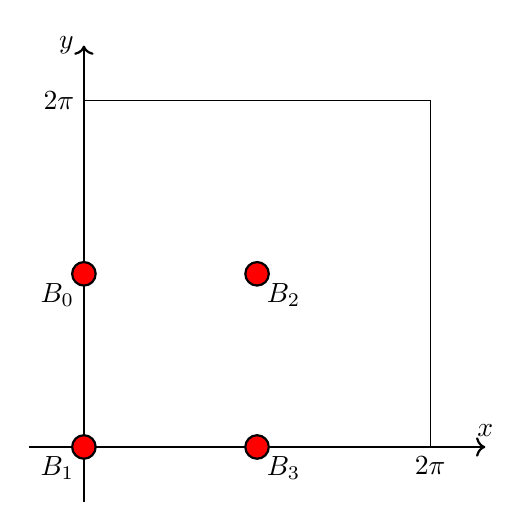
\begin{tikzpicture}[scale=0.7, vertex/.style={draw,circle,thick,fill=red,inner sep=3pt}]
\draw[->,thick] (-1,0) -- (2*pi+1,0) node[above] {$x$};
\draw[->,thick] (0,-1) -- (0,2*pi+1) node[left] {$y$};
\draw (0,0) rectangle (2*pi,2*pi);

\draw (2*pi,0) node[below] {$2\pi$};
\draw (0,2*pi) node[left] {$2\pi$};

\draw (0,0) node[vertex] {} node[below left] {$B_1$};
\draw (0,pi) node[vertex] {} node[below left] {$B_0$};
\draw (pi,0) node[vertex] {} node[below right] {$B_3$};
\draw (pi,pi) node[vertex] {} node[below right] {$B_2$};
\end{tikzpicture}
\caption{The periodic orbits of $H_1$ and their actions and Maslov indices}
\label{fig:po1}
\end{figure}

The actions of these orbits can be easily computed by direct application of the formula. We organize their actions in a line, forming the so-called \emph{action spectrum}, which will be important shortly.

\begin{figure}[H]
\centering
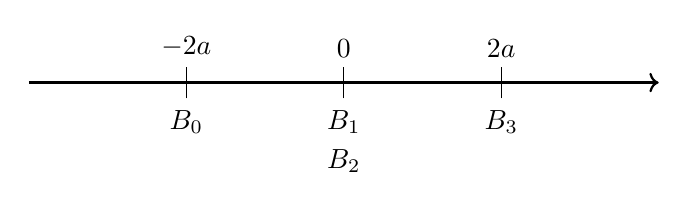
\begin{tikzpicture}[xscale=2]
\draw[->,thick] (-2.000,0.000)--(2.000,0.000);
\draw[] (-1.000,-0.200)--(-1.000,0.200) node[above] {$-2a$};
\draw[] (0.000,-0.200)--(0.000,0.200) node[above] {$0$};
\draw[] (1.000,-0.200)--(1.000,0.200) node[above] {$2a$};

\node at (-1, -0.5) {$B_0$};
\node at (0,-0.5) {$B_1$};
\node at (0, -1.0) {$B_2$};
\node at (1,-0.5) {$B_3$};
\end{tikzpicture}
\caption{The action spectrum of $\phi$.}
\end{figure}

Now, let us begin computing the barcode of $\phi$. In truth, there is not one barcode but many, one for each integer value of $k$, and each orbit will contribute to either the creation or destruction of a bar. For example, since $B_0$ is the orbit with least action, it necessarily corresponds to the creation of a bar (because there are no bars to destroy). But the question remains about which barcode this bar starts in.

To answer this question it is necessary to know about something called the Maslov index of an orbit. This is an integer number which is associated to a periodic orbit $x$ of a Hamiltonian, and it is denoted $\mu(x)$. Roughly speaking, to compute $\mu(x)$ one writes $(\dl \phi_t)_x$ as a (time-dependent) matrix and calculates the so-called Conley-Zehnder index of this path of matrices.

The Conley-Zehnder index of a path of (symplectic) matrices has a rather technical definition (see e.g. chap. 7 of \cite{audin}), and it is not feasible in most cases to compute it by direct application of its definition. There are alternative definitions which are more amenable to computation but require certain regularity assumptions, as in \cite{robbin1993maslov}. Since these regularity assumptions do not hold for the paths of matrices necessary to compute $\mu(B_i)$, $i = 0,\dots, 3$, I had to find a feasible way to compute Conley-Zehnder indices which would work for the case at hand.

I now present the main result of my thesis in this respect. It is not without limitations, as it only works in the case of $2 \times 2$ matrices, but it was sufficient here given that the manifold in question is the two-dimensional torus. However, its power comes from that fact that it works directly with the entries of the matrix path, without need for something like spectral decomposition of the path of matrices.

\begin{prop}[Corollary 4]
Let $A(t)$, $t \in \interval 0 T$ be a path of matrices with $A(0) = I$ and $\trace A(T) \neq 2$.\footnote{We show that a matrix $A$ is in $Sp(2n)^*$ if and only if $\trace A \neq 2$.} If $\trace A(t) > -2$ for all time and $\trace A(T) > 2$, the Maslov index of $A$ is zero. Otherwise, there exists a partition of the form
\begin{equation}
0 = a_0 < b_0 < a_1 < b_1 < a_2 < \dots < a_N < b_N \leq T
\end{equation}
which satisfies the properties
\begin{enumerate}
\item $(-1)^n \trace A(a_n) \geq 2$,
\item $\trace A(b_n) \in \ointerval{-2}2$,
\item Whenever $\trace A(x) \geq 2$ and $\trace A(y) \leq -2$, there exists some $b_n$ between $x$ and $y$,
\item\label{calcmaslov:ab5} Exactly one of $\trace A(a_N)$ and $\trace A(T)$ is in $\rinterval 2 \infty$.
\end{enumerate}

For any such partition, we have the formula
\begin{equation}\label{calcmaslov:mu}
\mu(A(t)) = \sum (-1)^n \sign(A(b_n)_{12})
\end{equation}
\end{prop}

Using this proposition, it is possible to verify that $\mu(B_0) = -1$, $\mu(B_1) = \mu(B_2) = 0$, and $\mu(B_3) = 1$. As a consequence, we know that $B_0$ induces the creation of a bar at $-2a$, in the barcode of index $-1$.

Now, let us look at $B_1$ and $B_2$. Each of them could create a new bar or destroy the one which already exists, induced by $B_0$.\footnote{An orbit $x$ will either create a bar in the barcode of index $\mu(x)$, or destroy a bar in the barcode of index $\mu(x)-1$.} However, this is where the fact that filtered Floer homology agrees (for large $\lambda$) with the usual Floer homology, which in turn agrees with homology in the usual sense. Because of this, it is possible to verify that, at infinity, the barcode of $\phi$ will have exactly four bars. Consequently, for this particular barcode, as there are only four periodic orbits \emph{there can be no destruction of bars}. Therefore, both $B_1$ and $B_2$, as well as $B_3$, induce creation of bars at appropriate time on the appropriate barcode, and so the barcode of $\phi$ is given by the one in figure \ref{fig:bc1}.
\begin{figure}[H]
\centering
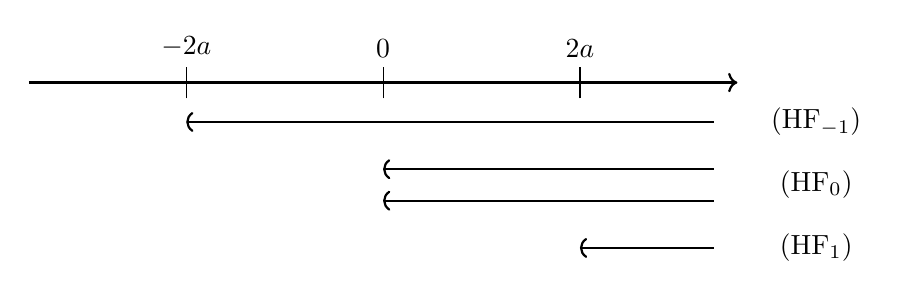
\begin{tikzpicture}
\draw[->,thick] (-4.500,0.000)--(4.500,0.000);
\draw[] (0.000,-0.200)--(0.000,0.200) node[above] {0};
\draw[] (2.500,-0.200)--(2.500,0.200) node[above] {$2a$};
\draw[] (-2.500,-0.200)--(-2.500,0.200) node[above] {$-2a$};
\draw[(-,thick] (-2.500,-0.500)--(4.200,-0.500);
\node[] at (5.500,-0.500) {$(\HF_{-1})$};
\draw[(-,thick] (0.000,-1.100)--(4.200,-1.100);
\draw[(-,thick] (0.000,-1.500)--(4.200,-1.500);
\node[] at (5.500,-1.300) {$(\HF_0)$};
\draw[(-,thick] (2.500,-2.100)--(4.200,-2.100);
\node[] at (5.500,-2.100) {$(\HF_1)$};
\end{tikzpicture}
\caption{The barcode of $\phi$.}\label{fig:bc1}
\end{figure}

To conclude, let us present a more complicated example. In the case of $\phi$, the appearance of the barcode does not depend qualitatively on the value of $a$ chosen, as long as $a > 0$. However, if we consider the diffeomorphism $\phi^2 = \phi \circ \phi$, this changes, with large numbers of periodic orbits appearing as $a \to \infty$.

In my thesis, I studied $\phi^2$ for values of the parameter $0 < a < \pi$. Within this range, there is a phase change at $a = 2$. For $a < 2$ the barcode is uninteresting, looking a lot like figure \ref{fig:bc1}, but for $2 < a < \pi$ we get more interesting results. We present a diagram with the contractible periodic orbits of $\phi^2$, as well as its barcode.

\begin{figure}[H]
\centering
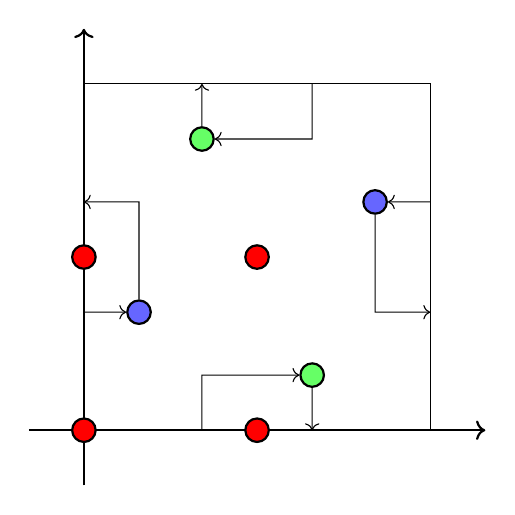
\begin{tikzpicture}[scale=0.7, vertex/.style={draw,circle,thick,fill=red,inner sep=3pt}]
\draw[->,thick] (-1,0) -- (2*pi+1,0);
\draw[->,thick] (0,-1) -- (0,2*pi+1);
\draw (0,0) rectangle (2*pi,2*pi);

\draw (0,0) node[vertex] {};
\draw (0,pi) node[vertex] {};
\draw (pi,0) node[vertex] {};
\draw (pi,pi) node[vertex] {};

\node[vertex,fill=blue!60] (A0) at (1,pi-1) {};
\node[vertex,fill=blue!60] (A1) at (2*pi-1,pi+1) {};
\draw[->] (0,pi-1) -- (A0);
\draw[->] (A0) -- (1,pi+1) -- (0,pi+1);
\draw[->] (2*pi,pi+1) -- (A1);
\draw[->] (A1) -- (2*pi-1,pi-1) -- (2*pi,pi-1);

\node[vertex,fill=green!60] (C0) at (pi+1,1) {};
\node[vertex,fill=green!60] (C1) at (pi-1,2*pi-1) {};
\draw[->] (C0) -- (pi+1,0);
\draw[->] (pi-1,0) -- (pi-1,1) -- (C0);
\draw[->] (C1) -- (pi-1,2*pi);
\draw[->] (pi+1,2*pi) -- (pi+1,2*pi-1) -- (C1);
\end{tikzpicture}
\caption{The eight contractible periodic orbits of $\phi^2$ ($2 < a < \pi$).}
\label{orbitsh12}
\end{figure}

\begin{figure}[H]
\centering
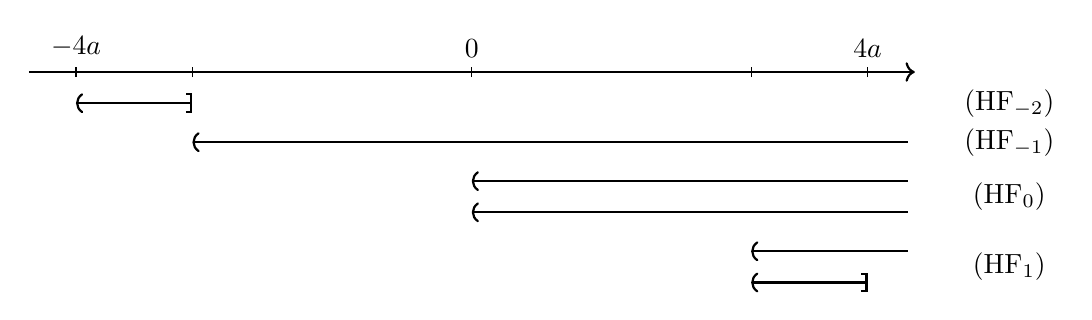
\begin{tikzpicture}[yscale=0.33, xscale=0.4]
\draw[->,thick] (-14.066,0.000)--(14.066,0.000);
\draw[] (0.000,-0.200)--(0.000,0.200) node[above] {0};
\draw[] (-12.566,-0.200)--(-12.566,0.200) node[above] {$-4a$};
\draw[] (12.566,-0.200)--(12.566,0.200) node[above] {$4a$};
\draw[] (-8.870,-0.200)--(-8.870,0.200);
\draw[] (8.870,-0.200)--(8.870,0.200);
\draw[{(-]},thick] (-12.566,-1.200)--(-8.870,-1.200) node[right] {};
\node[] at (17.066,-1.200) {$(\HF_{-2})$};
\draw[(-,thick] (-8.870,-2.700)--(13.841,-2.700) node[right] {};
\node[] at (17.066,-2.700) {$(\HF_{-1})$};
\draw[(-,thick] (0.000,-4.200)--(13.841,-4.200) node[right] {};
\draw[(-,thick] (0.000,-5.400)--(13.841,-5.400) node[right] {};
\node[] at (17.066,-4.800) {$(\HF_0)$};
\draw[(-,thick] (8.870,-6.900)--(13.841,-6.900) node[right] {};
\draw[{(-]},thick] (8.870,-8.100)--(12.566,-8.100) node[right] {};
\node[] at (17.066,-7.500) {$(\HF_{1})$};
\end{tikzpicture}
\caption{The barcode of the filtered Floer homology of $\phi^2$, for $2<a<\pi$.}
\end{figure}

\bibliographystyle{plain}
\bibliography{bibliography}

\end{document}